\documentclass[a4paper,14pt]{extreport}
	\usepackage[left=1.5cm,right=1.5cm,
	    top=1.5cm,bottom=2cm,bindingoffset=0cm]{geometry}
	\usepackage{scrextend}
	\usepackage[T1,T2A]{fontenc}
	\usepackage[utf8]{inputenc}
	\usepackage[english,russian,ukrainian]{babel}
	\usepackage{tabularx}
	\linespread{1.3}
	\usepackage{amssymb}
	\usepackage{fp}
	\usepackage{color}
	\usepackage{amsmath}
	\usepackage{mathrsfs}
	\usepackage{listings}
	\usepackage{graphicx}
	\graphicspath{ {./images/} }
	\usepackage{lipsum}
	\usepackage{xcolor}
	\usepackage{multirow}
	%\usepackage[table,xcdraw]{xcolor}
	\usepackage{hyperref}
	\usepackage{tcolorbox}
	\usepackage{tikz}
	\usepackage[framemethod=TikZ]{mdframed}
	\usepackage{wrapfig,boxedminipage,lipsum}
	\usepackage{tcolorbox}



\begin{document}
\newtcbox{\xmybox}[1][red]{on line, arc=7pt,colback=#1!10!white,colframe=#1!50!black, before upper={\rule[-3pt]{0pt}{10pt}},boxrule=1pt, boxsep=0pt,left=6pt,right=6pt,top=2pt,bottom=2pt}

\begin{titlepage}
	\begin{center}
	\large
	Національний технічний університет України \\ "Київський політехнічний інститут імені Ігоря Сікорського"


	Факультет Електроніки

	Кафедра мікроелектроніки
	\vfill

	\textsc{ЗВІТ}\\

	{\Large Про виконання лабораторної роботи №3\\
	з дисципліни: «Функціональна електроніка»\\[1cm]

	Дослідження логічних схем на тунельних діодах


	}
	\bigskip
	\end{center}
	\vfill

	\newlength{\ML}
	\settowidth{\ML}{«\underline{\hspace{0.4cm}}» \underline{\hspace{2cm}}}
	\hfill
	\begin{minipage}{1\textwidth}
	Виконавець:\\
	Студент 4-го курсу \hspace{4cm} $\underset{\text{(підпис)}}{\underline{\hspace{0.2\textwidth}}}$  \hspace{1cm}А.\,С.~Мнацаканов\\


	Перевірила: \hspace{5.9cm} $\underset{\text{(підпис)}}{\underline{\hspace{0.2\textwidth}}}$  \hspace{1cm}Т.\,Ю.~Обухова\\

	\end{minipage}

	\vfill

	\begin{center}
	2021
	\end{center}
\end{titlepage}






\textbf{Мета роботи} -Дослідження принципів роботи логічних схем на тунельних діодах.
\begin{center}
\textbf{Порядок виконання роботи}
\end{center}
	\begin{enumerate}
	\item Ввімкнути джерело живлення логічних схем і осцилограф. 
	\item Підключити логічну схему A до джерела живлення і до осцилографа. 
	\item  Перевести перемикачі вхідних сигналів у положення «0». 
	\item  Ввімкнути схему. 
	\item  Виставити необхідну комбінацію вхідних сигналів і визначити за показами осцилографа відповідне логічне значення на виході схеми. 
	\item  Вимкнути схему. 
	\item  Повторити п.3-6 для кожної комбінації вхідних сигналів. 
	\item  Відключити осцилограф та джерело живлення від логічноії схеми A і підключити їх до логічної схеми B. 
	\item  Повторити п.3-7 для логічної схеми B. 
	\item  Вимкнути осцилограф і джерело живлення логічних схем і відключити їх від логічної схеми B. 
	\item  Отримати у викладача варіант завдання на розрахунок логічної схеми.
	\end{enumerate}

\begin{figure}[h!]
	\center{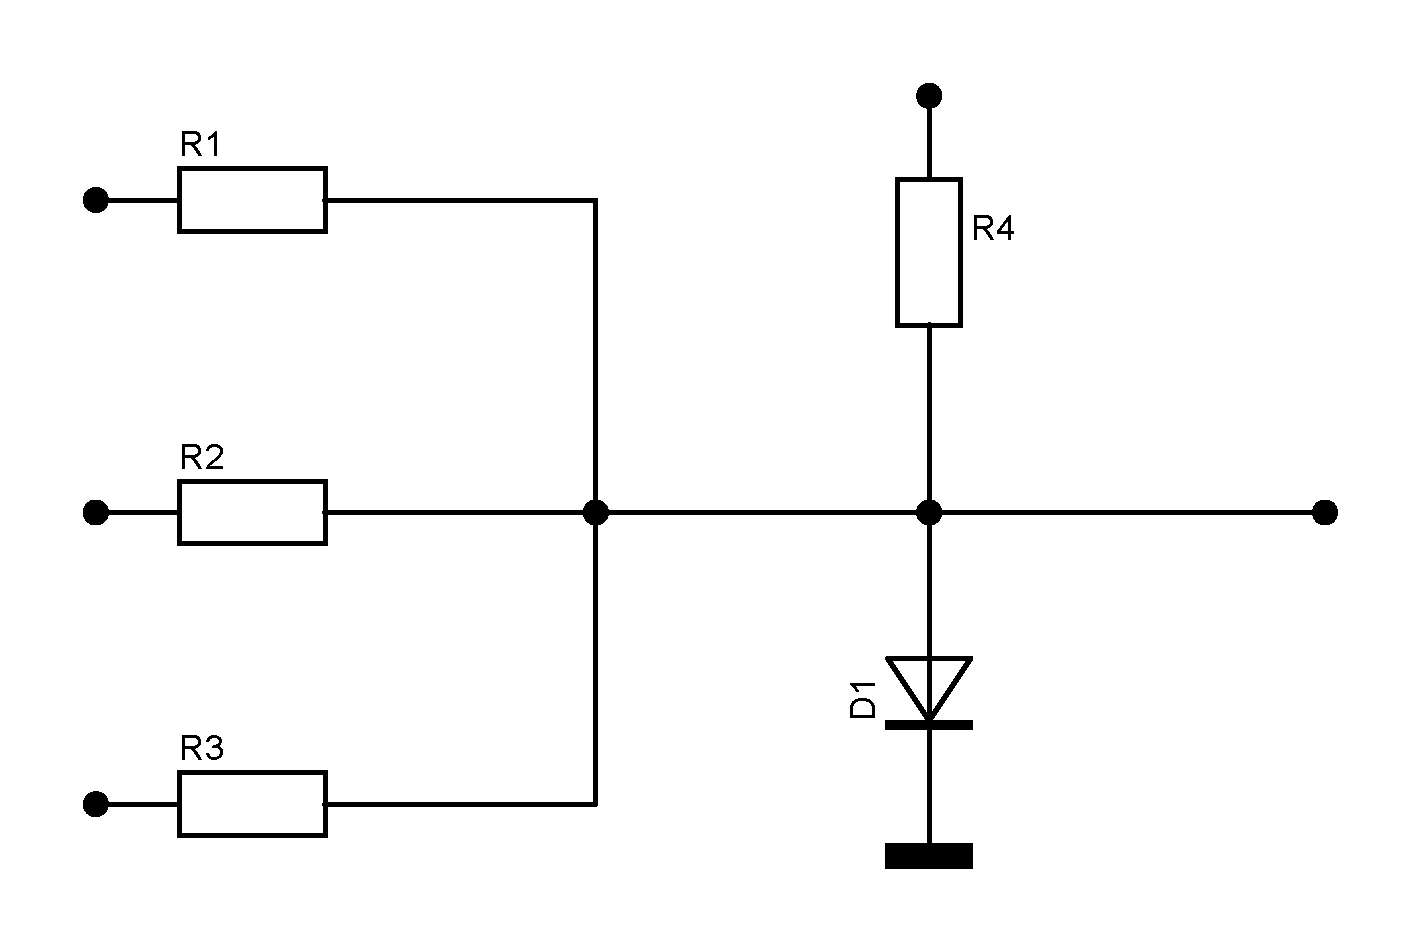
\includegraphics[width=0.4\linewidth]{picture1.pdf}}
	\caption{Принципова схема для логічної функції «АБО» на тунельному діоді.}
	\label{ris1}
\end{figure}

\newpage

\begin{center}
\textbf{Обробка результатів}
\end{center}
\begin{minipage}{0.35\textwidth}
\begin{tcolorbox}[ title=\textbf{Дано (варіант 13)}]
$U_{\text{жив}}= 1 B$\\
$U_{n_1}= 2 B$\\
$I_n = 2 \text{мА}$\\
$U_{n}= 0,18 B$\\
$I_{\text{в}} = 0,25 \text{мА}$\\
$U_{\text{B}}= 0,4 B$\\
$U_{\text{P}}= 0,75 B$\\
\end{tcolorbox}
\end{minipage}
\hfill
\begin{minipage}{0.6\textwidth}
\begin{center}Розрахунок\end{center}
$I_{\text{н}} + I_{R} \ge I_{\text{піку}}$\\

$R_{n} = \dfrac{U_{\text{н}}}{I_{\text{н}}} = \dfrac{1}{0,5} = 2\cdot 10^{3}$ = 2 кОм.\\

$I_{R_2} = 1,6 $ мА\\

$\dfrac{U_{\text{н}}}{I_{\text{н}}} = R \Rightarrow R = 625 $ Ом



\end{minipage}








\end{document}